
% This LaTeX was auto-generated from MATLAB code.
% To make changes, update the MATLAB code and republish this document.

\documentclass{article}
\usepackage{graphicx}
\usepackage{color}

\sloppy
\definecolor{lightgray}{gray}{0.5}
\setlength{\parindent}{0pt}

\begin{document}

    
    

\section*{27. $\hbox{Pad\'e}$ approximation}

\begin{verbatim}
ATAPformats
\end{verbatim}
\begin{par}

Suppose $f$ is a function with a Taylor series
$$ f(z) = c_0 + c_1 z + c_2 z^2 + \cdots \eqno (27.1) $$
at $z=0$.\footnote{This chapter is
adapted from Gonnet, G\"uttel and Trefethen [2012].}
Whether or not the series converges doesn't matter in this
chapter (it is enough for $f$ to be a {\em formal power series}). For any
integer $m\ge 0$, the {\em \boldmath degree $m$ Taylor approximant} to
$f$ is the unique polynomial $p_m\in{\cal P}_m$ that matches the series
as far as possible, which will be at least through degree $m$,
$$ (f - p_m)(z) = O(z^{m+1}). \eqno (27.2) $$
Pad\'e approximation is the
generalization of this idea to rational approximation.  For any integers
$m,n \ge 0$, $r\in {\cal R}_{mn}$ is the {\em type $(m,n)$
Pad\'e approximant} to $f$ if their Taylor series at $z=0$ agree as far
as possible:
$$ (f- r_{mn})(z)  = O(z^{\hbox{\footnotesize\rm maximum}}).
\eqno (27.3) $$
In these conditions the ``big O'' notation has its usual precise meaning.
Equation (27.2) asserts, for example, that the first nonzero
term in the Taylor series for $f-p_m$ is of order $z^k$ for some
$k\ge m+1$, but not necessarily $k=m+1$.

\end{par} \vspace{1em}
\begin{par}

Pad\'e approximation can be viewed as the special case of
rational interpolation in which the interpolation points coalesce at a
single point.
Thus there is a close analogy between the mathematics of
the last chapter and this one, though some significant differences too
that spring from the fact that the powers $z^0, z^1, \dots$ are
ordered whereas the roots of unity are all equal in status.
We shall see that a key property is that
$r_{mn}$ exists and is unique.  Generically, it matches
$f$ through term $m+n$,
$$ (f- r_{mn})(z) = O(z^{m+n+1}),
\eqno (27.4) $$
but in some cases, the matching will be to lower or higher order.

\end{par} \vspace{1em}
\begin{par}
For example, the type $(1,1)$ $\hbox{Pad\'e}$ approximant to $e^z$ is $(1+\textstyle{1\over 2}z)/(1-\textstyle{1\over 2}z)$, as we can verify numerically with the Chebfun command \texttt{padeapprox}:
\end{par} \vspace{1em}
\begin{par}
 \vskip -2em 
\end{par} \vspace{1em}
\begin{verbatim}
[r,a,b] = padeapprox(@exp,1,1);
fprintf('    Numerator coeffs: %19.15f %19.15f\n',a)
fprintf('  Denominator coeffs: %19.15f %19.15f\n',b)
\end{verbatim}

        \color{lightgray} \begin{verbatim}    Numerator coeffs:   1.000000000000000   0.500000000000000
  Denominator coeffs:   1.000000000000000  -0.500000000000000
\end{verbatim} \color{black}
    \begin{par}
The algorithm used by \texttt{padeapprox} will be discussed in the second half of this chapter.
\end{par} \vspace{1em}
\begin{par}

The early history of Pad\'e approximation is hard to disentangle because
every continued fraction can be regarded as a Pad\'e approximant (Exercise 27.7),
and continued fractions got a lot of attention in past centuries.
For example, Gauss derived the idea of Gauss quadrature from a continued
fraction that amounts to a Pad\'e approximant to the function
$\log((z+1)/(z-1))$ at the point $z=\infty$ [Gauss 1814, Takahasi \& Mori
1971, Trefethen 2008].  Ideas related to Pad\'e approximation have been credited to
Anderson (1740),
Lambert (1758) and Lagrange (1776), and contributions were certainly
made by Cauchy [1826] and Jacobi [1846].  The study of
Pad\'e approximants began to come closer to the current form with the
papers of Frobenius [1881] and
Pad\'e himself [1892], who was a student of
Hermite and published many articles
after his initial thesis on the subject.
Throughout the early literature, and also in the more recent era,
much of the discussion of Pad\'e approximation
is connected with continued fractions, determinants, and
recurrence relations, but here we shall follow a more robust matrix formulation.

\end{par} \vspace{1em}
\begin{par}

We begin with a theorem about existence, uniqueness, and
characterization, analogous to Theorem 24.1 for rational best
approximation on an interval.  There, the key idea was to count points of
equioscillation of the error function $f-r$.  Here, we count how many
initial terms of the Taylor series of $f-r$ are zero.  The arguments are
similar, and again, everything depends on the integer known as the
defect. Recall that if $r\in {\cal R}_{mn}$ is of exact type $(\kern
1pt\mu,\nu)$ for some $\mu\le m$, $\nu \le n$, then the defect of $r$
with respect to ${\cal R}_{mn}$ is $d = \min\{m-\mu, n-\nu\}\ge 0$, with
$\mu=-\infty$ and $d=n$ in the special case $r=0$.

\end{par} \vspace{1em}
\begin{par}

{\em {\bf Theorem 27.1: Characterization of Pad\'e approximants.}
For each $m,n\ge 0$, a function $f$ has a unique Pad\'e approximant
$r_{mn} \in {\cal R}_{mn}$ as defined by the condition $(27.3)$, and a
function $r \in {\cal R}_{mn}$ is equal to $r_{mn}$ if and only if
$(\kern .5pt f-r)(z) = O(z^{m+n+1-d\kern .5pt})$, where $d$ is the defect
of $r$ in ${\cal R}_{mn}$.}

\end{par} \vspace{1em}
\begin{par}

{\em Proof.}  The first part of the argument is analogous to parts 2 and
4 of the proof of Theorem 24.1: we show that if $r$ satisfies $(\kern
.5pt f-r)(z) = O(z^{m+n+1-d\kern .5pt})$, then $r$ is the unique type
$(m,n)$ Pad\'e approximant to $f$ as defined by the condition (27.3).
Suppose then that $(\kern .5pt f-r)(z) = O(z^{m+n+1-d\kern .5pt})$ and
that $(\kern .5pt f-\tilde r)(z) = O(z^{m+n+1-d\kern .5pt})$ also for
some possibly different function $\tilde r\in {\cal R}_{mn}$. Then
$(r-\tilde r)(z) = O(z^{m+n+1-d\kern .5pt})$. However, $r-\tilde r$ is of
type $(m+n-d, 2n-d\kern .7pt )$, so it can only have $m+n-d$ zeros at
$z=0$ unless it is identically zero.  This implies $\tilde r = r$.

\end{par} \vspace{1em}
\begin{par}

The other half of the proof is to show that there exists a
function $r$ with $(\kern .5pt f-r)(z) = O(z^{m+n+1-d\kern .5pt})$. This
part of the argument makes use of linear algebra and is given in the two
paragraphs following (27.8).
$~\hbox{\vrule width 2.5pt depth 2.5 pt height 3.5 pt}$

\end{par} \vspace{1em}
\begin{par}
Let us consider some examples to illustrate the characterization of Theorem 27.1.  First, a generic case, we noted above that the type (1,1) $\hbox{Pad\'e}$ approximant to $e^z$ is $r_{11}(z) = (1+\textstyle{1\over 2}z)/(1-\textstyle{1\over 2}z)$. The defect of $r_{11}$ in ${\cal R}_{11}$ is $d=0$, and we have $$ r_{11}(z) - e^z = \textstyle{1\over 12}z^3 + \textstyle{1\over 12} z^4 + \cdots = O(z^3).  $$ Since $m+n+1-d = 3$, this confirms that $r_{11}$ is the $\hbox{Pad\'e}$ approximant.
\end{par} \vspace{1em}
\begin{par}
On the other hand, if $f$ is even or odd, we soon find ourselves in the non-generic case.  Suppose we consider $$ f(z) = \cos(z) = 1 - \textstyle{1\over 2} z^2 + \textstyle{1\over 24} z^4 - \cdots $$ and the rational approximation $$ r(z) = 1 - \textstyle{1\over 2} z^2 $$ of exact type $(2,0)$.  This gives $$ (f-r)(z) = O(z^4), ~ \ne O(z^5) . $$ By Theorem 27.1, this implies that $r$ is the $\hbox{Pad\'e}$ approximation to $f$ for four different choices of $(m,n)$: $(2,0)$, $(3,0)$, $(2,1)$, and $(3,1)$. With $(m,n)= (2,0)$, for example, the defect is $d=0$ and we need $(\kern .5pt f-r)(z) = O(z^{2+0+1-0}) = O(z^3)$, and with $(m,n)= (3,1)$, the defect is $d=1$ and we need $(\kern .5pt f-r)(z) = O(z^{3+1+1-1}) = O(z^4)$.  Both matching conditions are satisfied, so $r$ is the $\hbox{Pad\'e}$ approximant of both types $(2,0)$ and $(3,1)$. Similarly it is also the $\hbox{Pad\'e}$ approximant of types $(3,0)$ and $(2,1)$, but for no other values of $(m,n)$.
\end{par} \vspace{1em}
\begin{par}

This example involving an even function suggests the general situation.
In analogy to the Walsh table of Chapter 24, the {\em Pad\'e table} of a
function $f$ consists of the set of its Pad\'e approximants for various
$m,n\ge 0$ laid out in an array, with $m$ along the horizontal and $n$
along the vertical:
$$ \pmatrix{
r_{00} & r_{10}& r_{20} & \dots \cr
r_{01} & r_{11}& r_{21} & \dots \cr
r_{02} & r_{12}& r_{22} & \dots \cr
\vdots & \vdots & \vdots & \ddots}. $$
The idea of the Pad\'e table was proposed by Pad\'e [1892], who called it
``a table of approximate rational fractions$\dots$ analogous to the
multiplication table, unbounded to the right and below.'' Like the Walsh
table for real rational approximation on an interval,
the Pad\'e table breaks into square blocks of degenerate entries,
again as a consequence of the equioscillation-type characterization
[Trefethen 1987]:

\end{par} \vspace{1em}
\begin{par}

{\em {\bf Theorem 27.2. Square blocks in the Pad\'e table.} The Pad\'e
table for any function $f$ breaks into precisely square blocks containing
identical entries.  (If $f$ is rational, one of these will be infinite in
extent.) The only exception is that if an entry $r=0$ appears in the
table, then it fills all of the columns to the left of some fixed index
$m = m_0$.}

\end{par} \vspace{1em}
\begin{par}
\textit{Proof.} Essentially the same as the proof of Theorem 24.2. $~\hbox{\vrule width 2.5pt depth 2.5 pt height 3.5 pt}$
\end{par} \vspace{1em}
\begin{par}
As in the case of best real approximation on an interval discussed in Chapter 24, square blocks and defects have a variety of consequences for $\hbox{Pad\'e}$ approximants.  In particular, the $\hbox{\em Pad\'e approximation operator}$, which maps Taylor series $f$ to their $\hbox{Pad\'e}$ approximants $r_{mn}$, is continuous at $f$ with respect a norm based on Taylor coefficients if and only if $r_{mn}$ has defect $d=0$. Another related result is that best supremum-norm approximations on intervals $[-\varepsilon,\varepsilon]$ converge to the $\hbox{Pad\'e}$ approximant as $\varepsilon\to 0$ if $d=0$, but not, in general, if $d> 0$. These results come from [Trefethen \& Gutknecht 1985], with earlier partial results due to Walsh; Werner and Wuytak; and Chui, Shisha and Smith.
\end{par} \vspace{1em}
\begin{par}
At this point we have come a good way into the theory of $\hbox{Pad\'e}$ approximation without doing any algebra.  To finish the job, and to lead into algorithms, it is time to introduce vectors and matrices, closely analogous to those of the last chapter.
\end{par} \vspace{1em}
\begin{par}

Given a function $f$ with Taylor coefficients $\{c_j\}$, suppose we look for
a representation of the Pad\'e approximant $r_{mn}$ as a quotient $r=p/q$
with $p\in {\cal P}_m$ and $q\in {\cal P}_n$. Equation (27.4) is
nonlinear, but multiplying through by the denominator suggests the linear
condition
$$ p(z) = f(z) q(z) +  O(z^{m+n+1}),
\eqno (27.5) $$
just as (26.4) led to (26.5).
To express this equation in matrix form, suppose that $p$ and $q$ are
represented by coefficient vectors $\bf a$ and ${\kern .5pt \bf b}$:
$$ {\bf a} = \pmatrix{a_0\cr a_1 \cr \vdots \cr a_m}, \qquad
{\kern .5pt \bf b} = \pmatrix{b_0\cr b_1 \cr \vdots \cr b_n}, $$
$$ p(z) = \sum_{k=0}^m a_kz^k, \qquad
q(z) = \sum_{k=0}^n b_kz^k. $$
Then (27.5) can be written as an equation involving a Toeplitz matrix of
Taylor coefficients of $f$,
that is, a matrix with constant entries along each diagonal.  For $m\ge
n$, the equation looks like this:
$$ \pmatrix{a_0\cr\noalign{\vskip 2pt} a_1 \cr \vdots \cr a_n \cr \vdots \cr
a_m \rule[-.6em]{0pt}{1em}\cr \hline \cr a_{m+1}\cr  \vdots
\cr a_{m+n}} =
\pmatrix{c_0\cr\noalign{\vskip 2pt}
c_1 & c_0 \cr
\vdots & \vdots & \ddots\cr
c_n & c_{n-1} & \dots & c_0 \cr
\vdots & \vdots &  & \vdots \cr
c_m & c_{m-1} & \dots & c_{m-n} \rule[-.6em]{0pt}{1em}\cr
\hline\cr
c_{m+1} & c_{m} & \dots & c_{m+1-n} \cr
\vdots & \vdots & \ddots & \vdots \cr
c_{m+n} & c_{m+n-1} & \dots & c_m
}
\pmatrix{b_0\cr b_1 \cr \vdots \cr b_n} \eqno (27.6) $$
coupled with the condition
$$ a_{m+1} = \cdots = a_{m+n} = 0. \eqno (27.7) $$
In other words, ${\kern .5pt \bf b}$ must be a null vector of the
$n\times(n+1)$ matrix displayed below the horizontal line.  If $m<n$,
the equation looks like this:
$$ \pmatrix{a_0\cr\noalign{\vskip 2pt} a_1 \cr \vdots \cr
a_m \rule[-.6em]{0pt}{1em}\cr \hline \cr a_{m+1}\cr  \vdots \cr a_n \cr
\vdots \cr a_{m+n}} =
\pmatrix{c_0\cr\noalign{\vskip 2pt}
c_1 & c_0 \cr
\vdots & \vdots & \ddots\cr
c_m & c_{m-1} & \dots & c_0 &  &   \rule[-.6em]{0pt}{1em}\cr
\hline\cr
c_{m+1} & c_{m} & \dots & c_1 & c_0 & \cr
\vdots & \vdots & & & \ddots & \ddots \cr
c_n & c_{n-1} & & \ddots & & c_1 & c_0 & \cr
\vdots & \vdots & & & &        & \vdots \cr
c_{m+n} & c_{m+n-1} & & \dots & & & c_m
}
\pmatrix{b_0\cr b_1 \cr \vdots \cr b_n}. $$
For simplicity we shall use the label (27.6) to refer to both cases,
writing the $n\times (n+1)$ matrix always as
$$ C  = \pmatrix{
c_{m+1} & c_m & \dots & c_{m+1-n} \cr
\vdots & \vdots & \ddots & \vdots \cr
c_{m+n} & c_{m+n-1} & \dots & c_m } \eqno (27.8) $$
with the convention that $c_k=0$ for $k<0$.

\end{par} \vspace{1em}
\begin{par}

One solution to (27.6)--(27.7) would be ${\bf a} = {\bf 0}$ and ${\kern
.5pt \bf b} = {\bf 0}$, corresponding to the useless candidate $r = 0/0$.
However, an $n\times (n+1)$ matrix always has a nonzero null vector,
$$ C \kern .7pt {\bf b\kern .5pt} = {\bf 0}, \quad
{\bf b\kern .5pt}\ne {\bf 0}, $$
and once ${\kern .5pt \bf b}$ is chosen, the coefficients $a_0,\dots ,
a_m$ of $p$ can be obtained by multiplying out the matrix-vector product
above the line. Thus there is always a solution to (27.5) with $q\ne 0$.

\end{par} \vspace{1em}
\begin{par}

If $b_0\ne 0$, then dividing (27.5) by $q$ shows that $p/q$ is a solution
to (27.4).  Some nonzero null vectors ${\kern .5pt \bf b}$, however, may
begin with one or more zero components.  Suppose that ${\kern .5pt \bf
b}$ is a nonzero null vector with $b_0 = b_1 = \cdots = b_{\sigma-1} = 0$
and $b_\sigma\ne 0$ for some $\sigma \ge 1$.  Then the corresponding
vector $\bf a$ will also have $a_0 = a_1 = \cdots = a_{\sigma-1} = 0$
(and $a_\sigma$ might be zero or nonzero).  It follows from the Toeplitz
structure of (27.6) that we can shift both $\bf a$ and ${\kern .5 pt \bf
b}$ upward by $\sigma$ positions to obtain new vectors ${\bf \tilde a} =
(a_\sigma,\dots,a_m,0,\dots,0)^T$ and ${\kern .5 pt \bf \tilde b} =
(b_\sigma,\dots,b_n,0,\dots,0)^T$ while preserving the quotient $r =
\tilde p/\tilde q = p/q$.  Thus $r$ has defect $d\ge \sigma$, and
equations (27.6)--(26.7) are still satisfied except that $\tilde
a_{m+n-\sigma+1},\dots, \tilde a_{m+n}$ may no longer be zero, implying
$(f-r)(z) = O(z^{m+n+1-\sigma})$. Thus $(f-r)(z) = O(z^{m+n+1-d})$, and
this completes the proof of Theorem 27.1.

\end{par} \vspace{1em}
\begin{par}
We have just shown that any nonzero null vector of the matrix $C$ of (27.8) gives a function $r$ that satisfies the condition for a $\hbox{Pad\'e}$ approximation, hence must be the unique approximant provided by Theorem 27.1.  So we have proved the following theorem.
\end{par} \vspace{1em}
\begin{par}

{\em{\bf Theorem 27.3.  Linear algebra solution of Pad\'e problem.} Given
a function $f$ with Taylor coefficients $\{c_j\}$, let\/ ${\bf b\kern
.5pt}$ be any nonzero null vector of the matrix\/ $C $ of\/ $(27.8)$,
let\/ ${\bf a}$ be the corresponding vector obtained from $(27.6)$, and
let\/ $p\in{\cal P}_m$ and\/ $q\in{\cal P}_n$ be the corresponding
polynomials. Then $r_{mn} = p/q$ is the unique type $(m,n)$ Pad\'e
approximant to $f$.}

\end{par} \vspace{1em}
\begin{par}
We emphasize that the vectors $\bf a$ and ${\kern .5pt \bf b}$ are not unique in general: a function in ${\cal R}_{mn}$ may have many representations $p/q$.  Nevertheless, all choices of $\bf a$ and ${\kern .5pt \bf b}$ lead to the same $r_{mn}$.
\end{par} \vspace{1em}
\begin{par}

From Theorems 27.1--27.3 one can derive a precise characterization of the
algebraic structure of the Pad\'e approximants to a function $f$, as
follows.  Let $\hat r$ be a rational function of exact type $(\kern
.5pt\mu,\nu)$ that is the Pad\'e approximant to $f$ in a
$(k+1)\times(k+1)$ square block for some $k\ge 0$:
$$ \pmatrix{r_{\mu\nu} & \dots & r_{\mu+k,\nu}  \cr\noalign{\vskip 3pt}
\vdots &  & \vdots \cr \noalign{\vskip 3pt}r_{\mu,\nu+k} & \dots  & r_{\mu+k,\nu+k}}. $$
Write $\hat r = \hat p/\hat q$ with $\hat p$ and $\hat q$ of
exact degrees $\mu$ and $\nu$.
From Theorem 27.1 we know that the defect $d$ must be distributed within
the square block according to this pattern illustrated for
$k=5$:
$$
\llap{\hbox{defect $d$:~~~}}\pmatrix{
0&0&0&0&0&0\cr
0&1&1&1&1&1\cr
0&1&2&2&2&2\cr
0&1&2&3&3&3\cr
0&1&2&3&4&4\cr
0&1&2&3&4&5}. \eqno (27.9)
$$
According to Theorem 27.3, the polynomials $p$ and $q$ that result
from solving the matrix problem (27.6)--(27.7) must be related to
$\hat p$ and $\hat q$ by
$$ p(z) = \pi(z) \hat p(z), \quad q(z) = \pi(z) \hat q(z) $$
for some polynomial $\pi$ of degree at most $d$. Now let us define the
{\bf deficiency} $\lambda$ of $r$ as the distance below the
cross-diagonal in the square block, with the following pattern:
$$
\llap{\hbox{deficiency $\lambda$:~~~}}\pmatrix{
0&0&0&0&0&0\cr
0&0&0&0&0&1\cr
0&0&0&0&1&2\cr
0&0&0&1&2&3\cr
0&0&1&2&3&4\cr
0&1&2&3&4&5}. \eqno (27.10)
$$
From Theorem 27.1, we know that in the positions of the block with
$\lambda>0$, $(f-r)(z) = O(z^{m+n+1-\lambda})$, $\ne
O(z^{m+n+2-\lambda})$, for otherwise, the block would be bigger.  For
this to happen, $\pi(z)$ must be divisible by $z^\lambda$, so that at
least $\lambda$ powers of $z$ are lost when solutions $p$ and $q$ from
(27.6) are normalized to $\hat p$ and $\hat q$.  Since $\pi$ may have
degree up to $d$, the number of degrees of freedom remaining in $p$ and
$q$ is $d-\lambda$, an integer we denote by $\chi$, distributed within
the block according to this pattern:
$$
\llap{\hbox{rank deficiency $\chi$:~~~}}\pmatrix{
0&0&0&0&0&0\cr
0&1&1&1&1&0\cr
0&1&2&2&1&0\cr
0&1&2&2&1&0\cr
0&1&1&1&1&0\cr
0&0&0&0&0&0}. \eqno (27.11)
$$
Thus the dimensionality of the space of vectors $q$ is $\chi+1$, and the
same for $p$. We call $\chi$ the {\em rank deficiency} of $r$ because of
a fact of linear algebra: the rank of the $n\times (n+1)$ matrix $C$ of
(27.8) must be equal to $n-\chi$, so that its space of null vectors will
have the required dimension $\chi+1$.  Some ideas related to these
developments can be found in [Heinig \& Rost 1984].

\end{par} \vspace{1em}
\begin{par}
We have just outlined a proof of the following theorem, which can be found in Section 3 of [Gragg 1972].
\end{par} \vspace{1em}
\begin{par}

{\em{\bf Theorem 27.4. Structure of a Pad\'e approximant.} Let $f$ and
$m,n\ge 0$ be given, let the type $(m,n)$ Pad\'e approximant $r_{mn}$ of
$f$ have exact type $(\kern .5pt \mu,\nu)$, and let $\hat p$ and $\hat
q\ne 0$ be polynomials of exact degrees $\mu$ and $\nu$ with $r_{mn} =
\hat p/\hat q$. Let the defect $d$, deficiency $\lambda$, and rank
deficiency $\chi = d-\lambda$ be defined as above. Then the matrix $C $
of $(27.8)$ has rank $n-\chi$, and two polynomials $p\in P_m$ and $q\in
P_n$ satisfy $(27.5)$ if and only if
$$
p(z) = \pi(z) \kern .7pt \hat p(z),
\quad q(z) = \pi(z)\kern .7pt  \hat q(z) \eqno (27.12)
$$
for some $\pi\in {\cal P}_d$ divisible by $z^\lambda$.}

\end{par} \vspace{1em}
\begin{par}
Although we did not state it in the last chapter, there is an analogue of this theorem for rational interpolation in distinct points, proved by Maehly and Witzgall [1960] and discussed also in [Gutknecht 1990] and $\hbox{[Pach\'on,}$ Gonnet \& Van Deun 2011].
\end{par} \vspace{1em}
\begin{par}
With the results of the past few pages to guide us, we are now prepared to talk about algorithms.
\end{par} \vspace{1em}
\begin{par}

At one level, the computation of $\hbox{Pad\'e}$ approximants is trivial,
just a matter of implementing the linear algebra of (27.6)--(27.7). In
particular, in the generic case, the matrix $C $ of (27.8) will have full
rank, and so will its $n\times n$ submatrix obtained by deleting the
first column. One computational approach to Pad\'e approximation is
accordingly to normalize $\kern .5pt \bf b$ by setting $b_0=1$ and then
determine the rest of the entries of {\bf b\kern .5pt} by solving a
system of equations involving this square matrix.

\end{par} \vspace{1em}
\begin{par}

This approach will fail, however, when the square matrix is singular, and
it is nonrobust with respect to rounding errors even when the matrix is
nonsingular.  To work with (27.8) robustly, it is a better idea to
normalize by the condition
$$ \| {\kern .5pt \bf b} \| = 1, $$
where $\|\cdot\|$ is the vector 2-norm, as in equation (26.6) of
the last chapter. We then
again consider the SVD (singular value decomposition) of $C $, a
factorization $$ C  = U \Sigma \kern .7pt V^*, \eqno (27.13) $$ where $U$
is $n\times n$ and unitary, $V$ is $(n+1)\times (n+1)$ and unitary, and
$\Sigma$ is an $n\times (n+1)$ real diagonal matrix with diagonal entries
$\sigma_1 \ge \sigma_2 \ge \cdots \ge \sigma_n \ge 0$.

\end{par} \vspace{1em}
\begin{par}
Suppose $\sigma_n>0$.  Then $C $ has rank $n$, and the final column of $V$ provides a unique nonzero null vector ${\kern .5pt \bf b}$ of $C$ up to a scale factor.  This null vector defines a polynomial $q\in {\cal P}_n$.  Moreover, from (27.11), we know that $(m,n)$ must lie on the outer boundary of its square block in the $\hbox{Pad\'e}$ table.  If $q$ is divisible by $z^\lambda$ for some $\lambda\ge 1$, then $(m,n)$ must lie in the bottom row or right column, and dividing $p$ and $q$ by $z^\lambda$ brings it to the left column or top row, respectively.  A final trimming of any trailing zeros in $p$ or $q$ brings them to the minimal forms $\hat p$ and $\hat q$ with exact degrees $\mu$ and $\nu$.
\end{par} \vspace{1em}
\begin{par}
On the other hand, suppose $\sigma_n = 0$, so that the number of zero singular values of $C$ is $\chi\ge 1$.  In this case (27.11) tells us that $(m,n)$ must lie in the interior of its square block at a distance $\chi$ from the boundary.  Both $m$ and $n$ can accordingly be reduced by $\chi$ and the process repeated with a new matrix and a new SVD, $\chi$ steps closer to the upper-left $(\kern .5pt \mu,\nu)$ corner.  After a small number of such steps (never more than $2+\log_2(d+1)$, where $d$ is the defect), convergence is guaranteed.
\end{par} \vspace{1em}
\begin{par}
These observations suggest the following SVD-based algorithm, introduced in [Gonnet, $\hbox{G\"uttel}$ \& Trefethen 2012].
\end{par} \vspace{1em}
\begin{par}

{\em {\sc Algorithm 27.1. Pure Pad\'e approximation in exact arithmetic}
\par\vskip 3pt
Input: $m\ge 0$, $n\ge 0$, and a vector {\bf c} of Taylor coefficients
$c_0,\dots,c_{m+n}$ of a function $f$.
\par\vskip 3pt
Output: Polynomials $p(z) = a_0+ \cdots + a_\mu z^\mu$ and
$q(z) = b_0+ \cdots + b_\nu z^\nu$, $b_0 = 1$, of the minimal degree type $(m,n)$
Pad\'e approximation of $f$.
\par\vskip 3pt
$1.$ If $c_0 = \cdots = c_m = 0$, set $p=0$ and $q=1$ and stop.
\par\vskip 3pt
$2.$ If\/ $n=0$, set $p(z) = c_0 + \cdots + c_mz^m$
and $q=1$ and go to Step\/~$8$.
\par\vskip 3pt
\hangindent=12pt $3.$ Compute the SVD\/ $(27.13)$ of the $n\times (n+1)$ matrix $C$.
Let $\rho\le n$ be the number of nonzero singular values.
\par\vskip 3pt
$4.$ If $\rho<n$,
reduce $n$ to $\rho$ and $m$ to $m-(n-\rho)$ and return to Step $2$.
\par\vskip 3pt
\hangindent=12pt $5.$  Get $q$ from the null right singular vector ${\kern .5pt \bf b}$ of
$C$ and then $p$ from the upper part of $(27.6)$.
\par\vskip 3pt
\hangindent=12pt $6.$ If $b_0=\cdots=b_{\lambda-1}=0$ for some $\lambda\ge 1$,
which implies also $a_0=\cdots=a_{\lambda-1}=0$,
cancel the common factor of $z^\lambda$ in $p$ and $q$.
\par\vskip 3pt
$7.$ Divide $p$ and $q$ by $b_0$ to
obtain a representation with $b_0=1$.
\par\vskip 3pt
$8.$ Remove trailing zero coefficients, if any,
from $p(z)$ or $q(z)$.}

\end{par} \vspace{1em}
\begin{par}
In exact arithmetic, this algorithm produces the unique $\hbox{Pad\'e}$ approximant $r_{mn}$ in a minimal-degree representation of type $(\kern 1pt \mu,\nu)$ with $b_0=1$. The greatest importance of Algorithm 27.1, however, is that it generalizes readily to numerical computation with rounding errors, or with noisy Taylor coefficients $\{c_j\}$.  All one needs to do is modify the tests for zero singular values or zero coefficients so as to incorporate a suitable tolerance, such as $10^{-14}$ for computations in standard 16-digit arithmetic.  The following modified algorithm also comes from [Gonnet, $\hbox{G\"uttel}$ \& Trefethen 2012].
\end{par} \vspace{1em}
\begin{par}

{\em {\sc Algorithm 27.2. Robust Pad\'e approximation for noisy data or
floating point arithmetic}
\par\vskip 3pt
Input: $m\ge 0$, $n\ge 0$, a vector {\bf c} of Taylor
coefficients $c_0,\dots,c_{m+n}$
of a function $f$, and a relative tolerance ${\tt tol} \ge 0$.
\par\vskip 3pt
Output: Polynomials $p(z) = a_0+ \cdots + a_\mu z^\mu$ and
$q(z) = b_0+ \cdots + b_\nu z^\nu$, $b_0=1$,
of the minimal degree type $(m,n)$
Pad\'e approximation of a function close to $f$.
\par\vskip 3pt
\hangindent=12pt $1.$  Rescale $f(z)$ to $f(z/\gamma)$ for some $\gamma>0$ if desired
to get a function whose Taylor coefficients
$c_0,\dots,c_{m+n}$ do not vary too widely.
\par\vskip 3pt
$2.$ Define $\tau = {\tt tol} \cdot \|{\bf c}\|_2$.
If $|c_0| = \cdots = |c_m| \le \tau,$ set $p=0$ and $q=1$ and stop.
\par\vskip 3pt
$3.$ If\/ $n=0$, set $p(z) = c_0 +\cdots + c_mz^m$ and $q = 1$
and go to Step\/~$7$.
\par\vskip 3pt
\hangindent=12pt $4.$ Compute the SVD\/ $(27.13)$ of the $n\times (n+1)$ matrix $C$.
Let $\rho\le n$ be the number of singular
values of $C$ that are greater than $\tau$.
\par\vskip 3pt
$5.$
If $\rho<n$, reduce $n$ to $\rho$ and $m$ to $m-(n-\rho)$
and return to Step $3$.
\par\vskip 3pt
\hangindent=12pt $6.$ Get $q$ from the null right singular vector $\kern .5pt \bf b$ of
$C$ and then $p$ from the upper part of $(27.6)$.
\par\vskip 3pt
\hangindent=12pt $7.$
If $|b_0|,\dots, |b_{\lambda-1}|\le{\tt tol}$ for some $\lambda\ge 1$,
zero the first $\lambda$ coefficients of $p$ and~$q$ and cancel
the common factor $z^\lambda$.
\par\vskip 3pt
\hangindent=12pt $8.$ If $|b_{n+1-\lambda}|,\dots, |b_n|\le{\tt tol}$ for some $\lambda\ge 1$,
remove the last $\lambda$ coefficients of~$q$.
If $|a_{m+1-\lambda}|,\dots, |a_m|\le\tau$ for some $\lambda\ge 1$,
remove the last $\lambda$ coefficients of~$p$.
\par\vskip 3pt
$9.$ Divide $p$ and $q$ by $b_0$ to
obtain a representation with $b_0=1$.
\par\vskip 3pt
\hangindent=17pt $10.$ Undo the scaling of Step~$1$ by redefining
$\gamma^j a_j$ as $a_j$ and $\gamma^j b_j$ as $b_j$ for each~$j$.\par}

\end{par} \vspace{1em}
\begin{par}

Algorithm 27.2 has been implemented in a Matlab code called {\tt
padeapprox} that is included in the Chebfun distribution, though it does
not involve chebfuns. In its basic usage, {\tt padeapprox} takes as
input a vector {\bf c} of Taylor coefficients together with a
specification of $m$ and $n$, with ${\tt tol} = 10^{-14}$ by default. For
example, following [Gragg 1972], suppose
$$ f(z) = {1-z+z^3\over 1-2z+z^2} =
1 + z + z^2 + 2z^3 + 3z^4 + 4z^5 + \cdots. $$ Then the type $(2,5)$
Pad\'e approximation of $f$ comes out with the theoretically correct
exact type $(0,3)$:

\end{par} \vspace{1em}
\begin{par}
 \vskip -2em 
\end{par} \vspace{1em}
\begin{verbatim}
c = [1 1 (1:50)];
[r,a,b] = padeapprox(c,2,5);
format short
disp('Coefficients of numerator:'), disp(a.')
disp('Coefficients of denominator:'), disp(b.')
\end{verbatim}

        \color{lightgray} \begin{verbatim}Coefficients of numerator:
     1
Coefficients of denominator:
    1.0000   -1.0000    0.0000   -1.0000
\end{verbatim} \color{black}
    \begin{par}

To illustrate the vital role of the SVD in such a calculation, here
is what happens if robustness is turned off by setting ${\tt tol}=0$:

\end{par} \vspace{1em}
\begin{par}
 \vskip -2em 
\end{par} \vspace{1em}
\begin{verbatim}
[r,a,b] = padeapprox(c,2,5,0);
disp('Coefficients of numerator:'), disp(a.')
disp('Coefficients of denominator:'), disp(b.')
\end{verbatim}

        \color{lightgray} \begin{verbatim}Coefficients of numerator:
   1.0e+16 *
    0.0000    0.0000    1.3312
Coefficients of denominator:
   1.0e+16 *
    0.0000   -0.0000    1.3312   -1.3312    0.0000   -1.3312
\end{verbatim} \color{black}
    \begin{par}
We now see longer vectors with enormous entries, on the order of the inverse of machine precision. The type appears to be $(2,5)$, but the zeros and poles reveal that this is spurious:
\end{par} \vspace{1em}
\begin{par}
 \vskip -2em 
\end{par} \vspace{1em}
\begin{verbatim}
format long g
disp('Zeros:'), disp(roots(a(end:-1:1)))
disp('Poles:'), disp(roots(b(end:-1:1)))
\end{verbatim}

        \color{lightgray} \begin{verbatim}Zeros:
      -1.42216212513465e-17 +    8.667108214078e-09i
      -1.42216212513465e-17 -    8.667108214078e-09i
Poles:
          -0.34116390191401 +      1.16154139999725i
          -0.34116390191401 -      1.16154139999725i
           0.68232780382802 +                     0i
      -1.42216212447289e-17 +    8.667108214078e-09i
      -1.42216212447289e-17 -    8.667108214078e-09i
\end{verbatim} \color{black}
    \begin{par}
We see that the two zeros are virtually cancelled by two poles that differ from them by only about $10^{-24}$.  Thus this approximant has two spurious pole-zero pairs, or Froissart doublets, introduced by rounding errors. Many $\hbox{Pad\'e}$ computations over the years have been contaminated by such effects, and in an attempt to combat them, many authors have asserted that it is necessary to compute $\hbox{Pad\'e}$ approximations in high precision arithmetic.
\end{par} \vspace{1em}
\begin{par}
If \texttt{padeapprox} is called with a Matlab function handle $f$ rather than a vector as its first argument, then it assumes $f$ is a function analytic in a neighborhood of the closed unit disk and computes Taylor coefficients by the Fast Fourier Transform. For example, here is the type $(2,2)$ $\hbox{Pad\'e}$ approximant of $f(z) = \cos(z)$:
\end{par} \vspace{1em}
\begin{par}
 \vskip -2em 
\end{par} \vspace{1em}
\begin{verbatim}
format long
[r,a,b] = padeapprox(@cos,2,2);
disp('Coefficients of numerator:'), disp(a.')
disp('Coefficients of denominator:'), disp(b.')
\end{verbatim}

        \color{lightgray} \begin{verbatim}Coefficients of numerator:
   1.000000000000000                   0  -0.416666666666667
Coefficients of denominator:
   1.000000000000000                   0   0.083333333333333
\end{verbatim} \color{black}
    \begin{par}
One appealing application of \texttt{padeapprox} is the numerical computation of block structure in the $\hbox{Pad\'e}$ table for a given function $f$. For example, here is a table of the computed pair $(\kern .5pt \mu,\nu)$ for each $(m,n)$ in the upper-left portion of the $\hbox{Pad\'e}$ table of $\cos(z)$ with $0\le m,n\le 8$.  One sees the $2\times 2$ block structure resulting from the evenness of $\cos(z)$.
\end{par} \vspace{1em}
\begin{par}
 \vskip -2em 
\end{par} \vspace{1em}
\begin{verbatim}
nmax = 8;
for n = 0:nmax
  for m = 0:nmax
    [r,a,b,mu,nu] = padeapprox(@cos,m,n); fprintf(' (%1d,%1d)',mu,nu)
  end
  fprintf('\n')
end
\end{verbatim}

        \color{lightgray} \begin{verbatim} (0,0) (0,0) (2,0) (2,0) (4,0) (4,0) (6,0) (6,0) (8,0)
 (0,0) (0,0) (2,0) (2,0) (4,0) (4,0) (6,0) (6,0) (8,0)
 (0,2) (0,2) (2,2) (2,2) (4,2) (4,2) (6,2) (6,2) (8,2)
 (0,2) (0,2) (2,2) (2,2) (4,2) (4,2) (6,2) (6,2) (8,2)
 (0,4) (0,4) (2,4) (2,4) (4,4) (4,4) (6,4) (6,4) (8,4)
 (0,4) (0,4) (2,4) (2,4) (4,4) (4,4) (6,4) (6,4) (8,4)
 (0,6) (0,6) (2,6) (2,6) (4,6) (4,6) (6,6) (6,6) (8,6)
 (0,6) (0,6) (2,6) (2,6) (4,6) (4,6) (6,6) (6,6) (8,6)
 (0,8) (0,8) (2,8) (2,8) (4,8) (4,8) (6,8) (6,8) (8,8)
\end{verbatim} \color{black}
    \begin{par}
We can also show the block structure with a color plot, like this:
\end{par} \vspace{1em}
\begin{par}
 \vskip -2em 
\end{par} \vspace{1em}
\begin{verbatim}
d = zeros(nmax+2);
rand('state',7); h = tan(2*rand(50)-1); h(8,1) = 1;
for n = 0:nmax, for m = 0:nmax
  [r,a,b,mu,nu] = padeapprox(@cos,m,n); d(n+1,m+1) = h(mu+1,nu+1);
end, end
pcolor(d), axis ij square off
\end{verbatim}

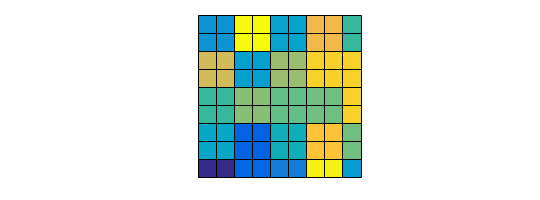
\includegraphics [width=4in]{chap27_01.png}
\begin{par}
 \vskip 1pt 
\end{par} \vspace{1em}
\begin{par}
The pattern of $2\times 2$ blocks is broken if we compute a larger segment of the table, such as $0\le m,n \le 16$:
\end{par} \vspace{1em}
\begin{par}
 \vskip -2em 
\end{par} \vspace{1em}
\begin{verbatim}
nmax = 16; d = zeros(nmax+2);
for n = 0:nmax, for m = 0:nmax
  [r,a,b,mu,nu] = padeapprox(@cos,m,n); d(n+1,m+1) = h(mu+1,nu+1);
end, end
pcolor(d), axis ij square off
\end{verbatim}

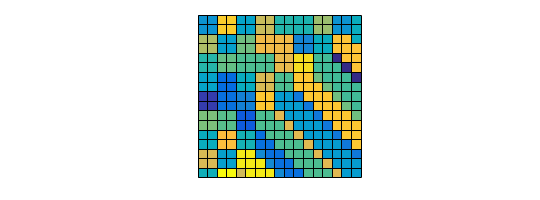
\includegraphics [width=4in]{chap27_02.png}
\begin{par}
 \vskip 1pt 
\end{par} \vspace{1em}
\begin{par}
What is going on here is that for $m+n$ greater than about $16$, $\cos(z)$ is resolved to machine precision, and the diagonal stripes of the plot show that \texttt{padeapprox} has automatically cut $m$ and $n$ down to this level.
\end{par} \vspace{1em}
\begin{par}
For an ``arbitrary'' function $f$ with gaps in its Taylor series, the block structure can be quite intriguing, as illustrated by this example with $f(z) = 1 + z + z^4 + z^7 + z^{10} + z^{13} + z^{16} + z^{17}$:
\end{par} \vspace{1em}
\begin{par}
 \vskip -2em 
\end{par} \vspace{1em}
\begin{verbatim}
nmax = 16; d = zeros(nmax+2);
f = @(z) 1+z+z.^4+z.^7+z.^10+z.^13.+z.^16+z.^17;
for n = 0:nmax, for m = 0:nmax
  [r,a,b,mu,nu] = padeapprox(f,m,n); d(n+1,m+1) = h(mu+1,nu+1);
end, end
pcolor(d), axis ij square off
\end{verbatim}

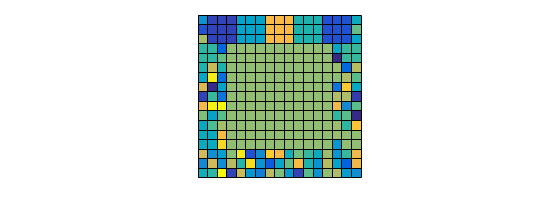
\includegraphics [width=4in]{chap27_03.png}
\begin{par}
 \vskip 1pt 
\end{par} \vspace{1em}
\begin{par}
Apart from $z^{17}$, these are the initial terms of the Taylor series of $$ f(z) = {1+z-z^3\over 1-z^3} , \eqno (27.14) $$ an example for which $\hbox{Pad\'e}$ worked out the block structure for $0\le m\le 7$, $0\le n \le 5$ $\hbox{[Pad\'e 1892],}$ showing vividly a $2\times 2$ block, two $3\times 3$ blocks, and the beginning of the infinite block at position $(3,3)$.
\end{par} \vspace{1em}
\begin{par}
In this chapter we have discussed how to compute $\hbox{Pad\'e}$ approximants, but not what they are useful for. As outlined in chapter 23, applications of these approximations typically involve situations where we know a function in one region of the $z$-plane and wish to evaluate it in another region that lies near or beyond certain singularities.  The next chapter is devoted to a practical exploration of such problems.
\end{par} \vspace{1em}
\begin{par}
From a theoretical perspective, a central question for more than a century has been, what sort of convergence of $\hbox{Pad\'e}$ approximants of a function $f$ can we expect as $m$ and/or $n$ increase to $\infty$? In the simplest case, suppose that $f$ is an entire function, that is, analytic for all $z$.  Then for any compact set $K$ in the complex plane, we know that the type $(m,0)$ $\hbox{Pad\'e}$ approximants converge uniformly on $K$ as $m\to\infty$, since these are just the Taylor approximants. One might hope that the same would be true of type $(m,n_0)$ approximants for fixed $n_0\ge 1$ as $m\to\infty$, or of type $(n,n)$ approximants as $n\to\infty$, but in fact, pointwise convergence need not occur in either of these situations. The problem is that spurious pole-zero pairs, Froissart doublets, may appear at seemingly arbitrary locations in the plane. As $m$ and/or $n$ increase, the doublets get weaker and their effects more localized, but they can never be guaranteed to go away.  (In fact, there exist functions $f$ whose $\hbox{Pad\'e}$ approximants have so many spurious poles that the sequence of $(n,n)$ approximants is unbounded for every $z\ne 0$ [Perron 1929, Wallin 1972].) The same applies if $f$ is meromorphic, i.e., analytic apart from poles, or if it has more complicated singularities such as branch points.  All this is in true in exact mathematics, and when there are rounding errors on a computer, the doublets become ubiquitous.
\end{par} \vspace{1em}
\begin{par}
Despite these complexities, important theorems have been proved. The theorem of de Montessus de Ballore [1902] concerns the case of $m\to \infty$ with fixed $n$, guaranteeing convergence in a disk about $z=0$ if $f$ has exactly $n$ poles there.  The Nuttall--Pommerenke theorem [Nuttall 1970, Pommerenke 1973] concerns $m = n \to \infty$ and ensures convergence for meromorphic $f$ not pointwise but \textit{in measure} or \textit{in capacity}, these being precise notions that require accuracy over most of a region as $m,n\to\infty$ while allowing for localized anomalies.  This result was powerfully generalized for functions with branch points by Stahl [1987], who showed that as $n\to \infty$, almost all the poles of type $(n,n)$ $\hbox{Pad\'e}$ approximants line up along branch cuts that have a property of minimal capacity in the $z^{-1}$-plane. For discussion of these results see [Baker \& Graves-Morris 1996]. There are also analogous results for multipoint $\hbox{Pad\'e}$ approximation and other forms of rational interpolation.  For example, an analogue of the de Montessus de Ballore theorem for interpolation as in the last chapter was proved by Saff [1972].
\end{par} \vspace{1em}
\begin{par}
As a practical matter, these complexities of convergence are well combatted by the SVD approach we have described, which can be regarded as a method of regularization of the $\hbox{Pad\'e}$ problem.
\end{par} \vspace{1em}
\begin{par}
For reasons explained in the last chapter, the whole discussion of this chapter has been based on the behavior of a function $f(z)$ at $z=0$ rather than this book's usual context of a function $f(x)$ on an interval such as $[-1,1]$.  There is an analogue of $\hbox{Pad\'e}$ approximation for $[-1,1]$ called $\hbox{\em Chebyshev--Pad\'e approximation}$, developed by Hornecker [1959], Maehly [1963], Frankel and Gragg [1973], Clenshaw and Lord [1974], and Geddes [1981].   The idea is to consider the analogue of (27.3) for Chebyshev series rather than Taylor series: $$ (f- r_{mn})(x)  = O(T_{\hbox{\footnotesize\rm maximum}}(x)). \eqno (27.14) $$ (The Maehly version starts from the analogue of the linearized form (27.5).) In analogy to Theorem 27.1, it turns out that any $r\in {\cal R}_{mn}$ satisfying $(\kern .5pt f-r)(x) = O(T_{m+n+1-d\kern .5pt}(x))$ is the unique $\hbox{Chebyshev--Pad\'e}$ approximant according to this definition, but now, there is no guarantee that such a function $r$ exists. For theoretical details, see [Trefethen \& Gutknecht 1987], and for computations in Chebfun, there is a code called \texttt{chebpade}.  As of today, there has not yet been a study of $\hbox{Chebyshev--Pad\'e}$ approximation employing the SVD-based robustness ideas described in this chapter for $\hbox{Pad\'e}$ approximation.
\end{par} \vspace{1em}
\begin{par}
For extensive information about $\hbox{Pad\'e}$ approximation, see the book by Baker and Graves-Morris [1996]. However, that monograph uses an alternative definition according to which a $\hbox{Pad\'e}$ approximant only exists if equation (27.4) can be satisfied, and in fact the present treatment is mathematically closer to the landmark review of Gragg [1972], which uses the definition (27.3).
\end{par} \vspace{1em}
\begin{par}

\begin{displaymath}
\framebox[4.7in][c]{\parbox{4.5in}{\vspace{2pt}\sl
{\sc Summary of Chapter 27.} Pad\'e approximation is the generalization
of Taylor polynomials to rational approximation, that is, rational
interpolation at a single point.  Pad\'e approximants are characterized by
a kind of equioscillation condition and can be computed
robustly by an algorithm based on the SVD.\ \ The analogue on the
interval $[-1,1]$ is known as Chebyshev--Pad\'e
approximation.\vspace{2pt}}}
\end{displaymath}

\end{par} \vspace{1em}
\begin{par}
\small
\parskip=2pt
\par
{\bf Exercise 27.1.  Pad\'e approximation of a logarithm.}  Show from Theorem 27.1 that the function
$f(z) = \log(1+z)$ has Pad\'e approximants $r_{00} = 0$,
$r_{1,0}(z) = z$, $r_{01}(z) = 0$, and $r_{11} = z/(1+\textstyle{1\over 2} z)$.
\par
{\bf Exercise 27.2.  Reciprocals and exponentials.}  (a) Suppose $r_{mn}$ is the
type $(m,n)$ Pad\'e approximant to a function $f$ with $f(0)\ne 0$.
Show that $1/r_{mn}$ is the type $(n,m)$ Pad\'e approximant to $1/f$.
(b) As a corollary, state a theorem relating the $(m,n)$ and $(n,m)$
Pad\'e approximants of $e^z$.
\par
{\bf Exercise 27.3. Prescribed block structures.}
Devise functions $f$ with the following structures in their
Pad\'e tables, and verify your claims numerically by color plots
for $0\le m,n \le 20$.
(a) $3\times 3$ blocks everywhere.
(b) $1\times 1$ blocks everywhere, except that $r_{11} = r_{21} = r_{12} = r_{22}$.
(c) $1\times 1$ blocks everywhere, except that all $r_{mn}$ with $n\le 2$ are the same.
\par
{\bf Exercise 27.4.  Order stars.}  The {\em order star} of a function
$f$ and its approximation $r$ is the set of points $z$ in the complex
plane for which $|f(z)| = |r(z)|$.  Use the Matlab {\tt contour} command
to plot the order stars of the Pad\'e approximations $r_{11}$, $r_{22}$,
$r_{32}$ and $r_{23}$ to $e^z$.  Comment on the behavior near the origin.
\par
{\bf Exercise 27.5. Nonsingularity and normality.}  Show that for a given
$f$ and $(m,n)$, the Pad\'e approximation $r_{mn}$ has defect $d=0$ if and
only if the square matrix obtained by deleting the first column of (27.8)
is nonsingular.  (If all such matrices are nonsingular, the Pad\'e table
of $f$ is accordingly {\bf normal}, with all its entries distinct.)
\par
{\bf Exercise 27.6.  Arbitrary patterns of square blocks?}
Knowing that degeneracies in the Pad\'e table always occupy square blocks,
one might conjecture that, given any tiling of
the quarter-plane $m\ge 0$, $n\ge 0$ by
square blocks, there exists a function $f$ with this pattern
in its Pad\'e table.  Prove that this conjecture is false.
(Hint: consider the case where the first two rows of the table are
filled with $2\times 2$ blocks [Trefethen 1984].)
\par
{\bf Exercise 27.7. Continued fractions and the Pad\'e table.}
If $d_0, d_1,\dots $ is a sequence of numbers, the {\em continued fraction}
$$ d_0 + {d_1z \over \displaystyle 1+{d_2z\over \displaystyle 1 + \cdots}} \eqno (27.15) $$
is a shorthand for the sequence of rational functions
$$ d_0, ~ d_0 + d_1z, ~ d_0 + {d_1z\over \displaystyle 1+d_2 z},~ \dots , \eqno (27.16) $$
known as {\em convergents} of the continued fraction.
(a) Show that if $d_0,\dots,d_{k-1}\ne 0$ and $d_k=0$, then (27.15) defines
a rational function $r(z)$, and determine its exact type.
(b) Assuming $d_k \ne 0$ for all $k$,
show that the convergents are the Pad\'e approximants of
types $(0,0), (1,0), (1,1), (2,1), (2,2), \dots$ of a certain formal
power series.

\end{par} \vspace{1em}



\end{document}
    
